% -*- coding: utf-8; -*-
\documentclass[11pt]{article}
\usepackage{hyperref}

\usepackage[brazilian]{babel}
\usepackage[utf8]{inputenc}
\usepackage[T1]{fontenc}
\usepackage{amsmath}
\usepackage{mathtools}
\usepackage{xcolor}
\usepackage[toc,page]{appendix}
\usepackage{float}
\usepackage{graphicx}
\usepackage{caption}
\usepackage{subcaption}

\title{\textbf{Relatório Projeto 2: Algorítimos para Big Data}}
\author{ \\ email: \href{mailto:@cin.ufpe.br}{vdcn@cin.ufpe.br}}
\author{Fernando Neto e Victor Di Cavalcanti Nicéas \\ email: \href{mailto:fbwn@cin.ufpe.br}{\{fbwn, vdcn\}@cin.ufpe.br}}
\date{22 de Agosto}

\usepackage{graphicx}

\begin{document}
\maketitle

\section{Identificação}
Identificação da equipe
\begin{itemize}
  \item Fernando Neto (~fbwn)
  \begin{itemize}
    \item Algorítimo \textbf{GK}
    \item \emph{Script} para realização do \emph{benchmark}
    \item \emph{Notebooks} para análise dos resultados
  \end{itemize}
  \item Victor Nicéas (~vdcn)
  \begin{itemize}
    \item Algorítimo \textbf{Q-Digest}
  \end{itemize}
\end{itemize}
\section{Implementação}
Neste projeto os algoritmos implementados foram o \textbf{GK} e o \textbf{Q-Digest}, ambos mantêm uma estrutura ordenada a qual permite responder a dois tipos de queries: \textbf{rank} e \textbf{quantil}.
\paragraph{Query Rank}
Neste primeiro tipo de query a estrutura de dados responde com a massa estimada de todos os elementos menores que o alvo da query. Assim temos o domínio composto por todos os elementos possíveis no Universo da estrutura e a imagem composta por inteiros entre zero e a massa total da estrutura.
\paragraph{Query Quantil}
Já nesta query o objetivo é, a partir de um valor \textbf{r}, estimas o elemento que tem rank compreendido dentro de uma determinada distância de \textbf{r}, esta distância será uma fração da massa total denominada \emph{epsilon}.


\subsection{GK}
O algoritmo GK é uma estrutura de lista cujos elementos são triplas $(x, g, \delta)$. Onde $x$ representa um elemento do conjunto original, $g$ é um inteiro que representa a quantidade de outros valores do conjunto original que são representados por esta tripla, já $\delta$ representa um grau de incerteza para os valores que estão contido na tripla. Assim a tripla $(10, 5, 3)$ é lida como o valor 10 representando outros 5 valores, menores ou iguais a 10, com grau de incerteza 3.

O algorítimo \textbf{GK} foi construído usando a linguagem de programação \textbf{Scala} e teve como referência a apresentação do tópico em aula, a secção 4.2 do livro \emph{Small Summaries for Big Data}, de \emph{Graham Cormode and Ke Yi}.

Utilizamos a estruturas de dados \textbf{List} nativa da linguagem. A escolha desta representação se deu principalmente por ser adequada para a utilização em funções recursivas, principalmente pelo mecanismo conhecido como \emph{patter matching}. A linguagem de programação escolhida também foi importante no desenho dos métodos que realizam as \emph{queries} devido às funções \emph{tail recursive} que garantem o controle da pilha de execução mesmo para recursões muito profundas. No caso específico dos testes para mensuração das métricas de \emph{baseline} foi este mecanismo que evitou o estouro da pilha. Nos casos onde usamos a classe \textbf{GK} a pilha não chegou a estourar, porém o uso da recursão de calda melhora a performance evitando trocas de contexto desnecessários.

A estrutura GK é composta de 3 métodos principais: \emph{update}, \emph{rank}, \emph{quantil}, cada um destes têm um método auxiliar ( \emph{updatePure}, \emph{query\_rank}, \emph{query\_quantil}) que visa facilitar execução de testes. Por fim temos a função \emph{compress} que é acionada a cada \emph{update} possivelmente reduzindo o tamanho da estrutura em um elemento.

Dentre as limitações notáveis podemos citar:

\begin{itemize}
  \item O código funciona apenas em modo \emph{batch}
  \item Debug de algumas situações que fugiam do esperado de acordo com as análises. Por exemplo: as \emph{query quantil} escapavam do limite de erro em alguns casos.
  \item Melhorar o escopo dos testes para garantir as propriedades esperadas da estrutura.
  \item Realizar análise de outros recursos do \emph{profiler}.
\end{itemize}

\subsection{Q-Digest}
    O algoritmo do Q-Digest propõe a quem usar-lo oferecer um \textit{bound} na quantidade de memória usada ao realizar \textit{queries} de \textbf{rank e quantil}. A entrada de uma stream de dados, consistindo de (x, w) refere-se ao \textit{elemento x} com \textit{peso w}, pode ser processada pelo Q-Digest de modo a facilitar as Queries. Operando sobre o universo [0 ... U-1], onde U é o número x máximo que o algoritmo irá processar. Cada elemento dentro desse universo será uma folha da árvore do Q-Digest, onde recursivamente será reunido informações sobre o intervalo dentro desse universo, afim de futuramente termos o refinamento de espaço. O que garante essa restrição é justamente a chamada periódica do compress, onde certos nós não precisam mais armazenar informação, já que é possivel somente consultar os ancestrais para queries de rank e de quantil.
    
    Foi construído em \textbf{C++}, tendo como referência e a apresentação do tópico em aula, a secção 4.1 do livro \emph{Small Summaries for Big Data}, de \emph{Graham Cormode and Ke Yi}. Inclusive, a implementação adotada no Q-Digest não foi a apresentada em aula, e sim dessa referência.

    Foi utilizado uma árvore binária para implementação do Q-Digest, usando paradigmas de orientação a objeto em c++. O calculo dos pesos da sub-árvore foi realizado através de um percorrimento na árvore e nehuma memória extra foi usada. O profiling de memória foi bastante básico, fazendo o cálculo de \textit{sizeof(Node) * numero-nodes}, onde o sizeof(Node) em c++ retorna a quantidade de memória reservada para um nó. Realizando a múltiplicação temos toda memória usada pela estrutura.

    O algoritmo \textit{compress} citado no livro foi interessante de observar seu comportamento. No livro, ele cita que a frequência do compress deveria ser feita \textit{from time to time}, mas não há nenhum estabelecimento formal da quantidade de vezes necessária chamar a função para que o seu bound do número de nós proposto seja de O(logU/epsilon). A quantidade de vezes que o compress foi chamado, no código implementado, foi a cada 100000 linhas do \textit{network-flows.csv}.

    

Dentre as limitações notáveis podemos citar:
\begin{itemize}
  \item Profiling mais preciso da memória usando massif.
  \item Melhorar implementação do quantil para não escaparem do limite de erro.
  \item Definir a constante de vezes que o compress precisa ser chamado e realizar a medição sobre a quantidade de vezes da chamada.
\end{itemize}

\section{Testes e Resultados}

\subsection{GK}

\subsubsection{Descrição do ambiente de testes}

O projeto foi compilado no seguinte ambiente:
\begin{itemize}
  \item OS: Devuan GNU/Linux Chimaera x86\_64
  \item Host: Inspiron 5570
  \item Kernel: 5.12.14-artix1-1
  \item CPU: Intel i5-8250U (8) @ 3.400GHz
  \item Memory: 154MiB / 7851MiB
\end{itemize}

Utilizando as seguintes ferramentas:
\begin{itemize}
  \item openjdk 11.0.12
  \item OpenJDK Runtime Environment (build 11.0.12+7-post-Debian-2)
  \item OpenJDK 64-Bit Server VM (build 11.0.12+7-post-Debian-2, mixed mode)
  \item SBT 1.5.5
  \item Scala 2.13.6
\end{itemize}

A execução dos testes foram realizados com os seguintes parâmetros para a JVM:
\begin{itemize}
  \item -J-Xms4096m : Memória inicial = 4 Gb
  \item -J-Xmx4096m : Memória máxima = 4 Gb
\end{itemize}

\subsubsection{Descrição dos experimentos realizados}
Inicialmente iremos apresentar um conjunto básico de parâmetros que terão o intuito de apresentar as ferramentas gráficas tornando assim a leitura inical menos densa. De forma complementar este conjunto inicial facilitou a construção dos \emph{scripts} de agregação e análise dos dados.

Inicialmente criamos uma classe chamada \emph{GKbaseline} a qual abstrai as funções que iremos utilizar tanto na estrutura de dados implementa (\textbf{GK}), quanto no cenário \emph{baseline}. Assim podemos controlar as execuções apenas via \emph{bash scripts}. Estes controlam os parâmetro:
\begin{itemize}
  \item target: $(0, 3, 4, 5, 6, 7)$
  \item epsilon: $(0;1)$
  \item is baseline? $[1 | 0]$
  \item is rank query? $[1 | 0]$
\end{itemize}
Como os resultados não são eventos aleatórios não realizamos repetições, apesar de que estas poderiam nos dar mais informações sobre o tempo de execução, por simplicidade preferimos não realiza-las. Desta forma o fluxo completo dos nossos testes é:

\begin{enumerate}
  \item Execução do gerador de experimentos

        Aqui geramos um arquivo com 100 queries aleatórias. No caso das \emph{rank queries} o universo é limitado pelo valor máximo sabido para aquele campo. Já para as \emph{quantiles queries} o limite é o número total de linhas no arquivo, ou seja, a massa total que a estrutura terá visto.

  \item Execução do baseline

        Neste passo registramos tempo de início e fim da execução do código e recebemos como saída: o tamanho final da estrutura e o tempo gastos para a execução das queries. Também são gerados dois arquivos com informações adicionais que iremos descrever em seguida.

  \item Execução do GK

        Idem

\end{enumerate}

\paragraph{Respostas às queries}
Após concluida a fase inicial, em que o arquivo de entrada é lido e são realizados todos os \emph{updates}, temos a estrutura pronta para ser consultada. Esta fase das consultas é disparada por um arquivo cuja direção é fornecida na invocação do \emph{GK}. Para cada \emph{query} sua resposta é guardada em um arquivo em separado. Para o caso dos \emph{quantis} guardamos não só a resposta como também uma consulta adicional ao \emph{rank} deste elemento. Assim podemos utilizar esta informação na nossa análise.

\paragraph{Profiler}
Para obter uma fotografia mais acurada do funcionamento da nossa implementação utilizamos o software \emph{async-profiler}\footnote{https://github.com/jvm-profiling-tools/async-profiler} para realizar amostras da execução e assim podemos inferir que trachos do código foram mais executado. O profiler é lançado juntamente com a invocação do nosso executável e registra o PID da JVM onde iremos executar nosso código. Assim no momento da análise podemos recuperar qual fração do tempo de CPU ocupada pela função \emph{update} e seus descendentes.


\subsubsection{Resultados}

A seguir apresentaremos os resultados de um cenário simples, apenas utilizando como parâmetros:
\begin{itemize}
  \item \emph{target}: 0 e 4
  \item \emph{epsilon}: 0.1 e 0.2
\end{itemize}

Nosso objetivo é simplificar a visualização e explicar nossas escolhas. Ao final voltaremos a apresentar gráfico semelhante cobrindo um espectro maior de parâmetro.


A seguir apresentamos os gráficos (\emph{boxplot}) para cada uma das métricas (predição, tempo, memória ram, espaço instanciado pelo \emph{sketch}), na sequência crescente dos targets. Em cada gráfico adicionamos uma linha azul indicando o valor do \emph{baseline}, no caso da predição o valor real para a variável alvo e nos demais casos a métrica referente à execução deste \emph{baseline}. na predição incluimos adicionalmente duas linhas vermelhas indicando os limites referentes à escolha do \emph{epsilon}, ou seja o valor real +- \emph{epsilon}. Na secção seguinte apresentaremos a discussão destes.
\newpage

\paragraph{Heat Map}

No primeiro conjunto de gráfico utilizamos a apresentação conhecida como mapa de calor onde temos basicamente um dado tabular que utiliza do espectro de cores para reforçar as amplitudes e ajudam à percepção de padrões. Neste caso estamos usando os parâmetros \emph{target} e \emph{epsilon} como variaveis independentes. E alternamos algums métricas como variável dependente, estes estão registradas nas legendas. Devido à quantidade de gráfico e à semelhança entre os resultados dos \emph{heatmaps} iremos apresentar apenas os resultantes da query do tipo quantil.


\begin{figure}[H]
  \centering
  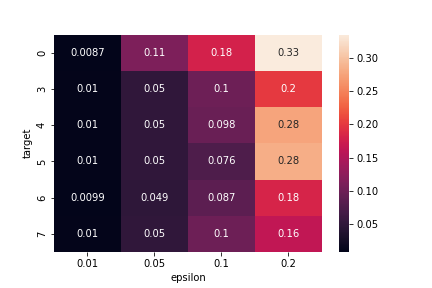
\includegraphics[scale=0.5]{../../img/QUANTIL_heatmap_ERRO.png}
  \caption{Erro médio para 100 consultas do tipo \emph{quantil}}
\end{figure}

\begin{figure}[ht]
\begin{subfigure}{.5\textwidth}
  \centering
  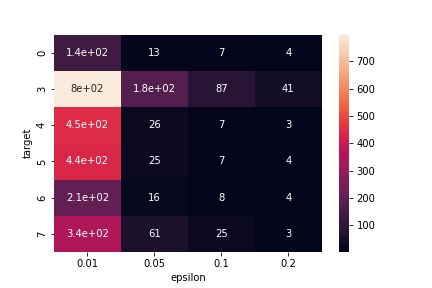
\includegraphics[width=.9\linewidth]{../../img/QUANTIL_heatmap_TAMANHO.png}
  \caption{Espaço utilizado pelo \newline GK: List[(Int,Int,Int)]}
  \label{fig:sub-first}
\end{subfigure}
\begin{subfigure}{.5\textwidth}
  \centering
  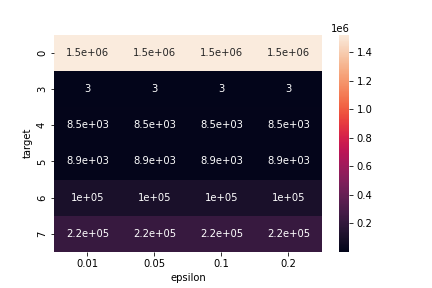
\includegraphics[width=.9\linewidth]{../../img/QUANTIL_heatmap_TAMANHO_BASELINE.png}
  \caption{Espaço utilizado pelo \newline baseline: SortedMap[Int,Int]}
\end{subfigure}
\caption{Tamanho das estruturas de dados}
\end{figure}


\begin{figure}[ht]
\begin{subfigure}{.5\textwidth}
  \centering
  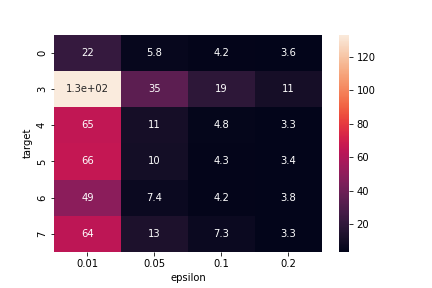
\includegraphics[width=.9\linewidth]{../../img/QUANTIL_heatmap_TEMPO_EXEC_SEG.png}
  \caption{GK}
  \label{fig:sub-first}
\end{subfigure}
\begin{subfigure}{.5\textwidth}
  \centering
  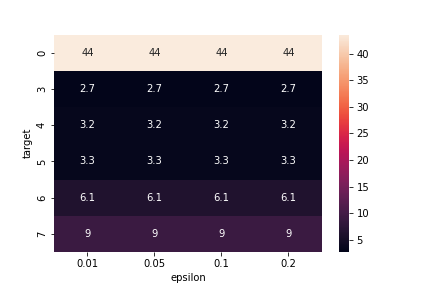
\includegraphics[width=.9\linewidth]{../../img/QUANTIL_heatmap_TEMPO_EXEC_SEG_BASELINE.png}
  \caption{Baseline}
\end{subfigure}
\caption{Tempo total de execução (segundos)}
\end{figure}


\begin{figure}[H]
\begin{subfigure}{.5\textwidth}
  \centering
  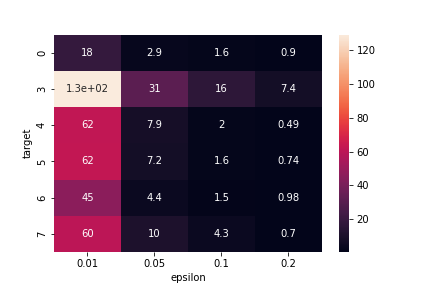
\includegraphics[width=.9\linewidth]{../../img/QUANTIL_heatmap_TEMPO_UPDATE.png}
  \caption{GK.update}
  \label{fig:sub-first}
\end{subfigure}
\begin{subfigure}{.5\textwidth}
  \centering
  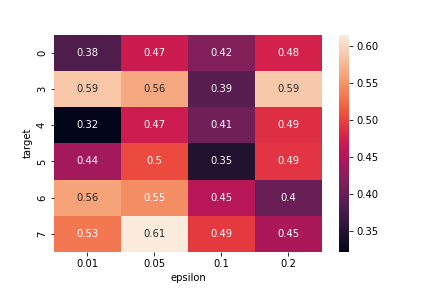
\includegraphics[width=.9\linewidth]{../../img/QUANTIL_heatmap_TEMPO_IO.png}
  \caption{java.io}
\end{subfigure}
\caption{GK: Update x IO (segundos)}
\end{figure}

\begin{figure}[H]
\begin{subfigure}{.5\textwidth}
  \centering
  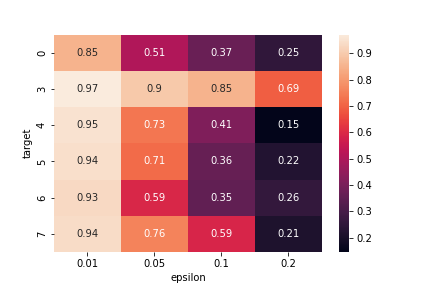
\includegraphics[width=.9\linewidth]{../../img/QUANTIL_heatmap_PROC_UPDATE.png}
  \caption{Update}
  \label{fig:sub-first}
\end{subfigure}
\begin{subfigure}{.5\textwidth}
  \centering
  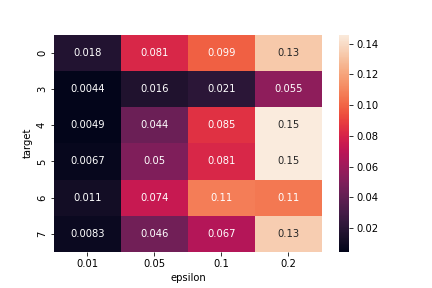
\includegraphics[width=.9\linewidth]{../../img/QUANTIL_heatmap_PROC_JAVAIO.png}
  \caption{IO}
\end{subfigure}
\caption{\% Ocupação da CPU: Update x IO (segundos)}
\end{figure}

\newpage

\subparagraph{Histogramas}

Uma caracteristica de estruturas ordenadas é a conservação da informação sobre a distribuição dos dados originais. Para verificar se a distribuição dos dados são semelhantes comparamos o histograma das queries no baseline (vermelho) com os resuldados no GK (verde).

\begin{figure}[H]
\begin{subfigure}{.5\textwidth}
  \centering
  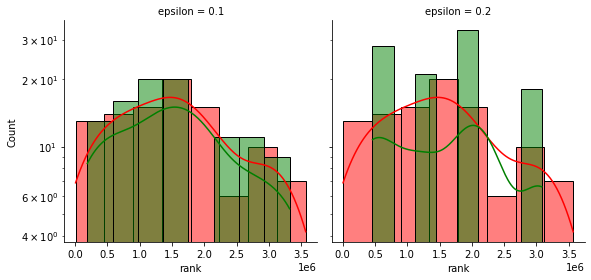
\includegraphics[width=.9\linewidth]{../../img/RANK_histograma_RANK_t_0.png}
  \caption{Target 0}
  \label{fig:sub-first}
\end{subfigure}
\begin{subfigure}{.5\textwidth}
  \centering
  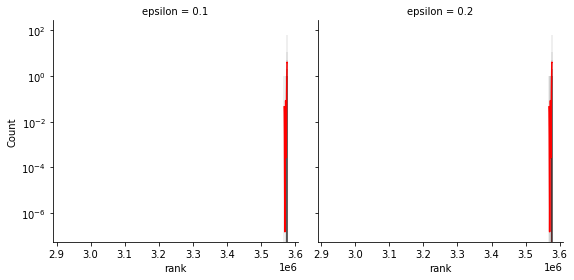
\includegraphics[width=.9\linewidth]{../../img/RANK_histograma_RANK_t_4.png}
  \caption{Target 4}
\end{subfigure}
\caption{Histogramas das queries do tipo \emph{rank}}
\end{figure}

\begin{figure}[H]
\begin{subfigure}{.5\textwidth}
  \centering
  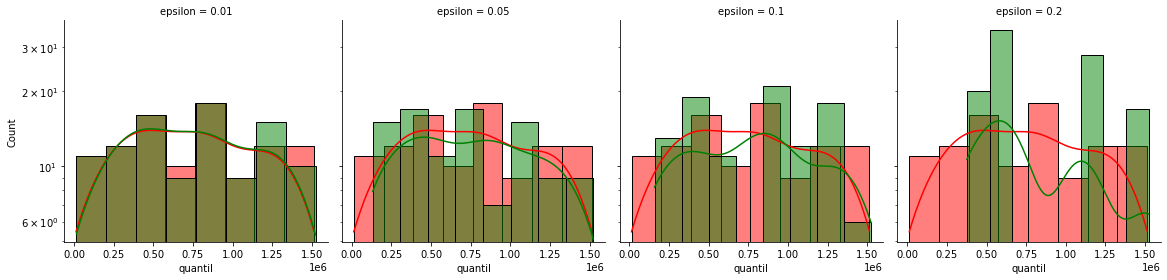
\includegraphics[width=.9\linewidth]{../../img/QUANTIL_histograma_distrib_QUANTIL_t_0.png}
  \caption{Target 0}
  \label{fig:sub-first}
\end{subfigure}
\begin{subfigure}{.5\textwidth}
  \centering
  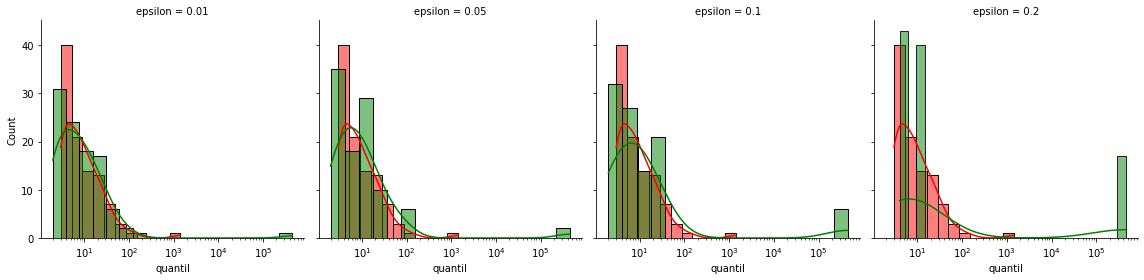
\includegraphics[width=.9\linewidth]{../../img/QUANTIL_histograma_distrib_QUANTIL_t_4.png}
  \caption{Target 4}
\end{subfigure}
\caption{Histogramas das queries do tipo \emph{quantil}}
\end{figure}

\subparagraph{Barras de Erro}

Nestas visualizações nosso objetivo é demonstrar que os resultados das consultas (verde) estão dentro da margem (vermelho) prometida pelo algoritmo em torno do valor real (laranja) extraído da execução do baseline.

\begin{figure}[H]
\begin{subfigure}{.5\textwidth}
  \centering
  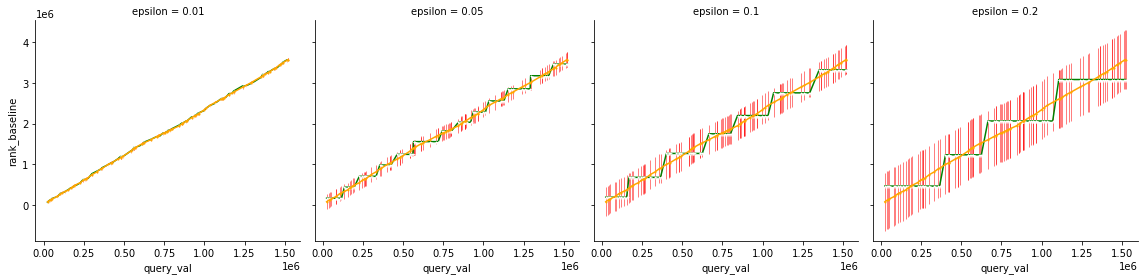
\includegraphics[width=.9\linewidth]{../../img/RANK_erroplot_ecdf_RANK_t_0.png}
  \caption{Target 0}
  \label{fig:sub-first}
\end{subfigure}
\begin{subfigure}{.5\textwidth}
  \centering
  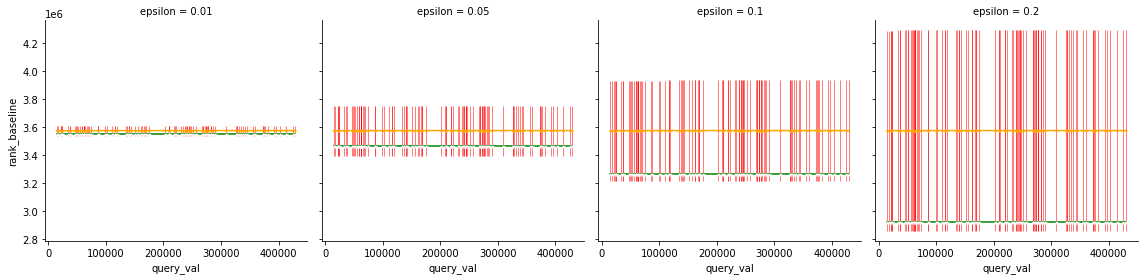
\includegraphics[width=.9\linewidth]{../../img/RANK_erroplot_ecdf_RANK_t_4.png}
  \caption{Target 4}
\end{subfigure}
\caption{Barras de erro das querie sdo tipo \emph{rank}}
\end{figure}

\begin{figure}[H]
\begin{subfigure}{.5\textwidth}
  \centering
  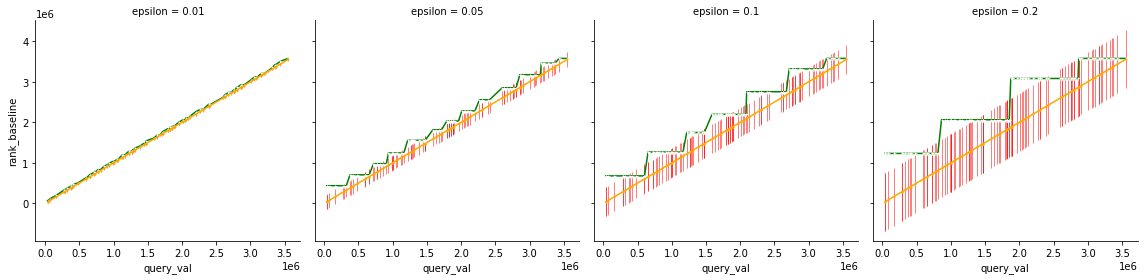
\includegraphics[width=.9\linewidth]{../../img/QUANTIL_erroplot_ecdf_QUANTIL_t_0.png}
  \caption{Target 0}
  \label{fig:sub-first}
\end{subfigure}
\begin{subfigure}{.5\textwidth}
  \centering
  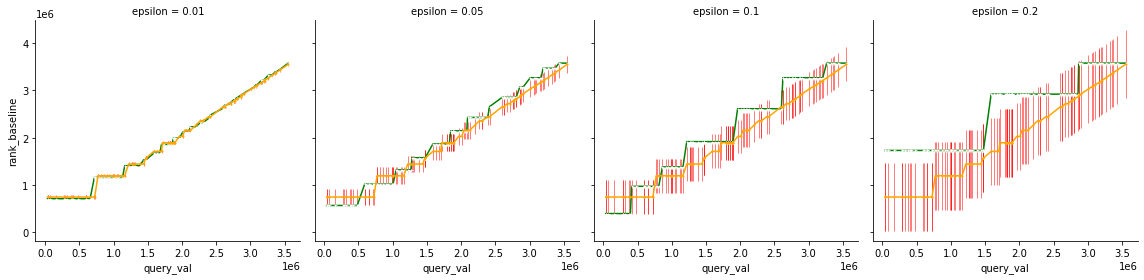
\includegraphics[width=.9\linewidth]{../../img/QUANTIL_erroplot_ecdf_QUANTIL_t_4.png}
  \caption{Target 4}
\end{subfigure}
\caption{Barras de erro das querie sdo tipo \emph{quantil}}
\end{figure}

\paragraph{Boxplot}

Por fim e complementando os gráficos de barras de erro temos o boxplot que sintetiza os erros de todas as 100 consultas para uma mesma estrutura (definida pelos parâmetros \emph{target, epsilon, query\_type})


\begin{figure}[H]
\begin{subfigure}{.5\textwidth}
  \centering
  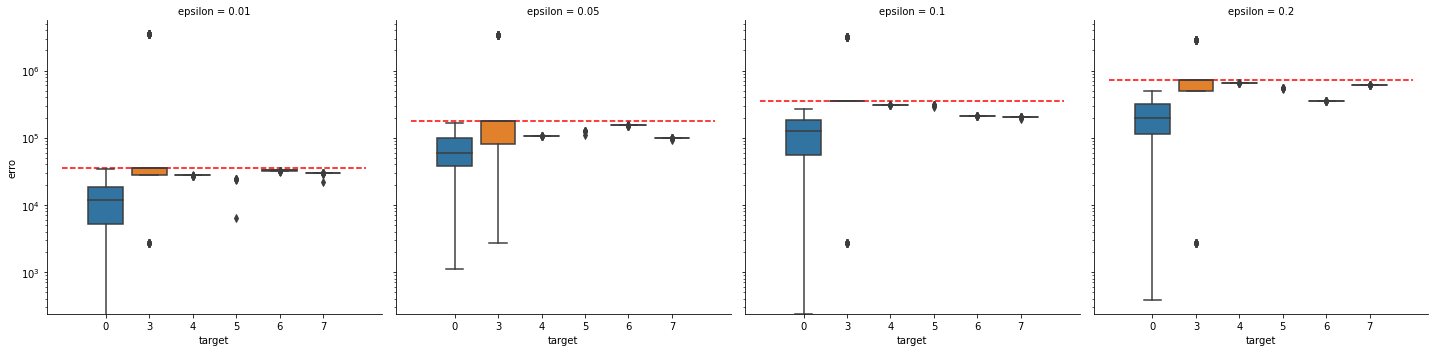
\includegraphics[width=.9\linewidth]{../../img/RANK_boxplot_erros.png}
  \caption{Query Rank}
  \label{fig:sub-first}
\end{subfigure}
\begin{subfigure}{.5\textwidth}
  \centering
  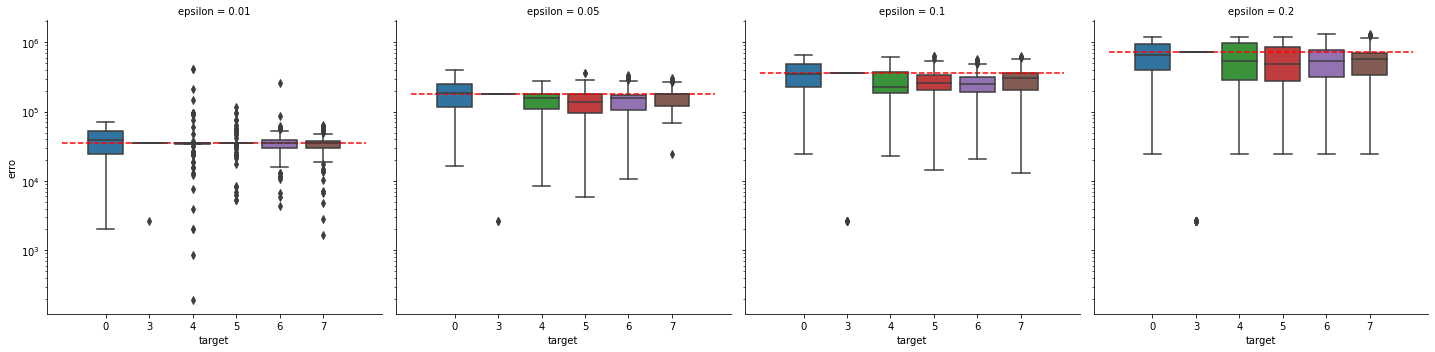
\includegraphics[width=.9\linewidth]{../../img/QUANTIL_boxplot_erros.png}
  \caption{Query Quantil}
\end{subfigure}
\caption{Boxplots}
\end{figure}



%%%%%%%%%%%%%%%%%%%
\subsubsection{Discussão dos resultados e conclusão}

\subsection{Q-Digest}
\subsubsection{Descrição do ambiente de testes}

O projeto foi compilado no seguinte ambiente:
\begin{itemize}
  \item OS: EndeavourOS Linux x86\_64
  \item Host: B450 AORUS PRO WIFI
  \item Kernel: 5.13.10-arch1-1
  \item CPU: AMD Ryzen 5 3500 (6) @ 3.600GHz
  \item Memory: 6048MiB / 15948MiB
\end{itemize}

Utilizando as seguintes ferramentas:
\begin{itemize}
  \item gcc version 11.1.0 (GCC)
  \item gperftools
  \item Python 3.9.6
\end{itemize}

\subsubsection{Descrição dos experimentos realizados}
Os experimentos foram de forma similar ao do GK. Algumas modificações ocorreram, como no Q-Digest precisamos do parâmetro do universo, foi pré computado o valor máximo que cada coluna.

Na implementação do Q-Digest, é feita a pré-alocação da árvore baseado no universo U. Para alguns valores, como \textit{target 6 e 7} a alocação passa do permitido pelo SO e o processo é morto. Foi feito a tentative de liberar mais memória para o processo, mas isso não ocorria. Uma solução para esse problema seria usar um \textit{bound} para o tamanho do universo, porém a precisão se compromete nesse aspecto. Foi criado diferentes \textit{scripts} para finalidade do experimento, como um para \textit{baseline rank, query rank e quantil}


Nos exemplos target 6 e 7 que foram feitos a análise de \textit{tempo}, utilizou-se um universo \emph{menor} do que o máximo representado na coluna. Não foi observado um erro não permitido na execução do programa.
\paragraph{Respostas às queries}
Às respostas as queries são feitas de forma idêntica ao do GK.

\paragraph{Profiler}
Foi feito experimentação usando a ferramente \textit{massif} que vem com valgrind e também a ferramente de profiling do google chamada gperftools. Com a gperftools, foi possível analisar a proporção de quanto a função ocupou do tempo de execução do código. Uma das limitações das ferramentas de profiling foi não se integrar com o batch de testes, tendo um exemplo de um caso único de análise de memória \textit{versus} execução do programa.

\subsubsection{Resultados}
A seguir apresentamos os resultados de um cenário com os seguintes targets e epsilons.
\begin{itemize}
  \item \emph{target}: 0, 3, 4, 5, 6, 7
  \item \emph{epsilon}: 0.01, 0.05, 0.1 e 0.2
\end{itemize}

\subparagraph{\emph{Query: Rank}}
\paragraph{Heat Map}
No heatmap, similar ao do GK, é possível visualizar o erro para cada target e epsilon respectivos.

\begin{figure}[H]
  \centering
  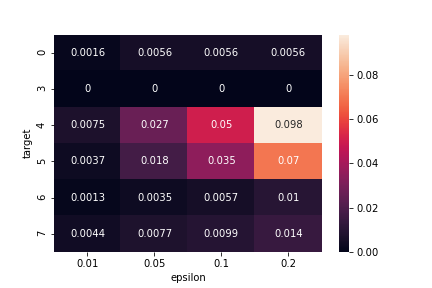
\includegraphics[scale=0.5]{../../img/qdigest-heatmap_ERRO.png}
  \caption{Erro médio para 100 consultas do tipo}
\end{figure}
O erro para o target 3 é um tanto problemático, já que é uma coluna bem polarizante com 2 valores distintos apenas.

\begin{figure}[H]
  \centering
  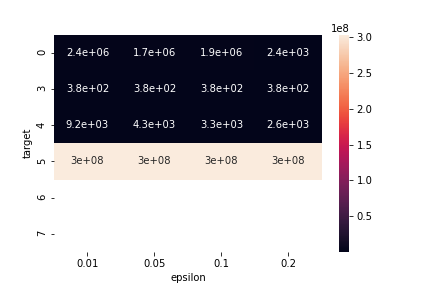
\includegraphics[scale=0.5]{../../img/qdigest-heatmap_MEM.png}
  \caption{Tamanho da estrutura de dados Q-Digest}
\end{figure}

Analisando a figura, como citado anteriormente, o target 6 e 7 estouraram a memória de execução. As execuções passadas conseguiram ser executados usando o bound máximo possível que consegue armazenar.

\begin{figure}[H]
  \centering
  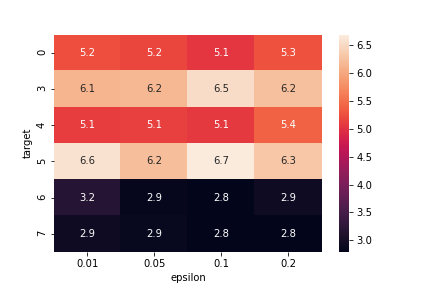
\includegraphics[scale=0.5]{../../img/qdigest-heatmap_TEMPO.png}
  \caption{Tamanho da estrutura de dados Q-Digest}
\end{figure}
O tempo de execução está em intervalos aceitáveis no que diz respeito a constante de tempo associada. Possíveis otimizações poderiam ser feito como não buscar semrpe o peso da sub-árvore realizando \textit{DFS} toda vez que precisar dessa informação.

\subparagraph{Histogramas}

Uma caracteristica de estruturas ordenadas é a conservação da informação sobre a distribuição dos dados originais. Para verificar se a distribuição dos dados são semelhantes comparamos o histograma das queries no baseline (vermelho) com os resuldados no Q-Digest (verde).
Alguns gráficos podem aparentar estarem distoantes o vermelho do verde, mas se observar bem a escala eles estão bem próximos.
\begin{figure}[H]
  \begin{subfigure}{.5\textwidth}
    \centering
    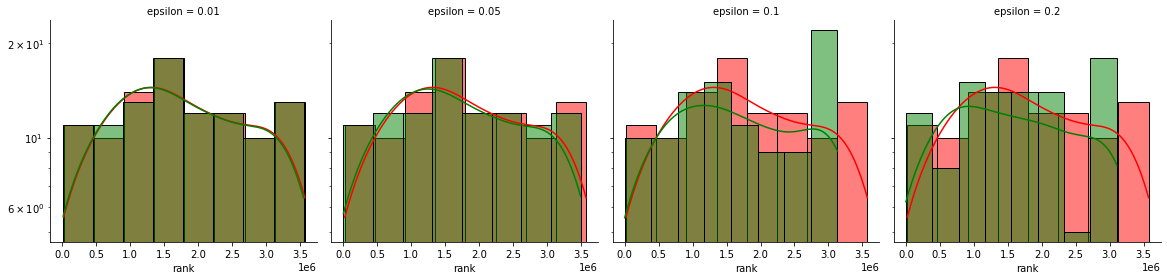
\includegraphics[width=.9\linewidth]{../../img/qdigest-histograma_distrib_RANK_t_0.png}
    \caption{Target 0}
    \label{fig:sub-first}
  \end{subfigure}
  \begin{subfigure}{.5\textwidth}
    \centering
    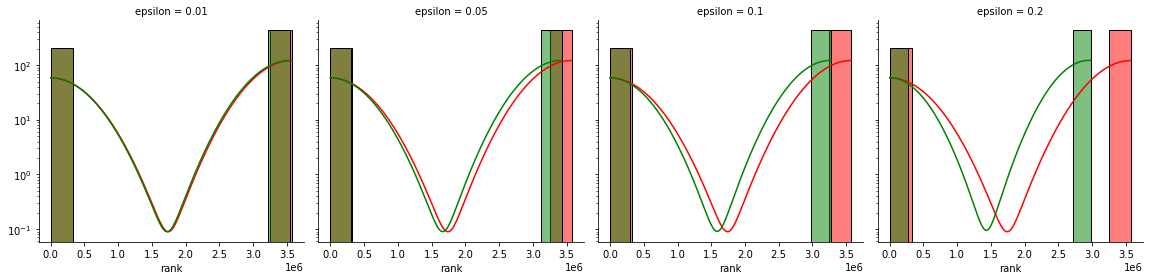
\includegraphics[width=.9\linewidth]{../../img/qdigest-histograma_distrib_RANK_t_3.png}
    \caption{Target 3}
  \end{subfigure}
  \caption{Histogramas das queries do tipo \emph{rank}}
  \end{figure}

  \begin{figure}[H]
    \begin{subfigure}{.5\textwidth}
      \centering
      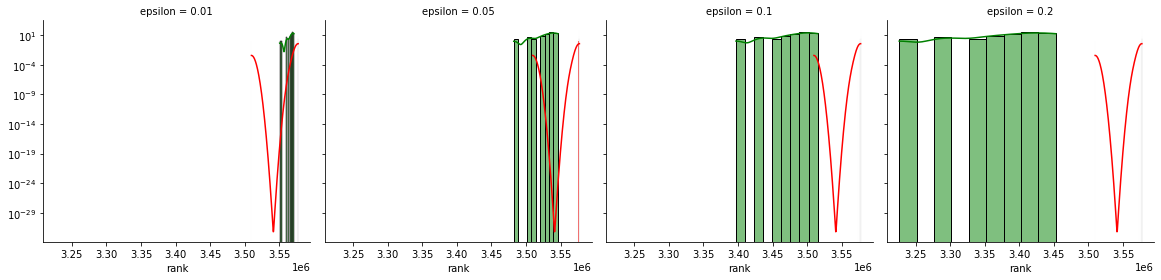
\includegraphics[width=.9\linewidth]{../../img/qdigest-histograma_distrib_RANK_t_4.png}
      \caption{Target 4}
      \label{fig:sub-first}
    \end{subfigure}
    \begin{subfigure}{.5\textwidth}
      \centering
      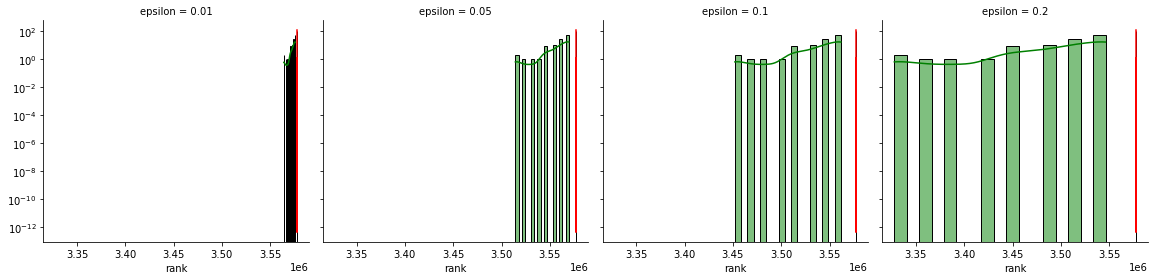
\includegraphics[width=.9\linewidth]{../../img/qdigest-histograma_distrib_RANK_t_5.png}
      \caption{Target 5}
    \end{subfigure}
    \caption{Histogramas das queries do tipo \emph{rank}}
    \end{figure}

    \begin{figure}[H]
      \begin{subfigure}{.5\textwidth}
        \centering
        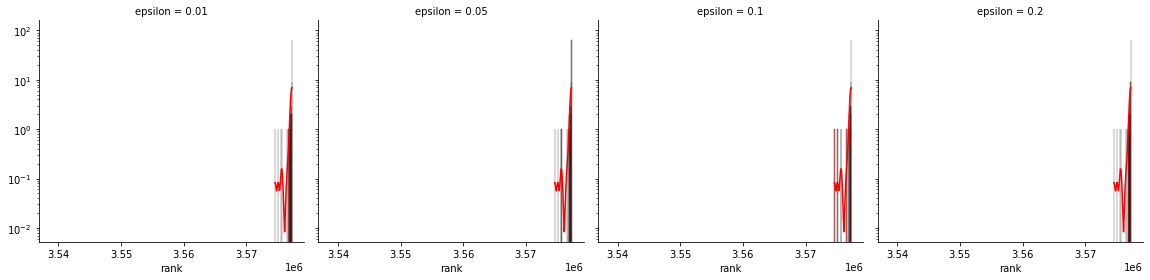
\includegraphics[width=.9\linewidth]{../../img/qdigest-histograma_distrib_RANK_t_6.png}
        \caption{Target 6}
        \label{fig:sub-first}
      \end{subfigure}
      \begin{subfigure}{.5\textwidth}
        \centering
        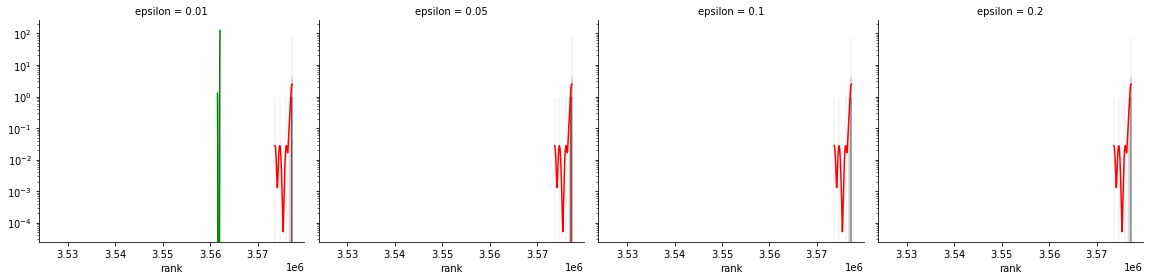
\includegraphics[width=.9\linewidth]{../../img/qdigest-histograma_distrib_RANK_t_7.png}
        \caption{Target 7}
      \end{subfigure}
      \caption{Histogramas das queries do tipo \emph{rank}}
      \end{figure}
      
    Como no Q-Digest, observamos que o parâmetro target 3 está saindo um pouco da correlação. Quanto maior a mistura de cores, mais fiel está ao baseline nossa distribuição dos dados.
    \subparagraph{Barras de Erro}
    Nestas visualizações nosso objetivo é demonstrar que os resultados das consultas (verde) estão dentro da margem (vermelho) prometida pelo algoritmo em torno do valor real (laranja) extraído da execução do baseline.
    
    \begin{figure}[H]
      \begin{subfigure}{.5\textwidth}
        \centering
        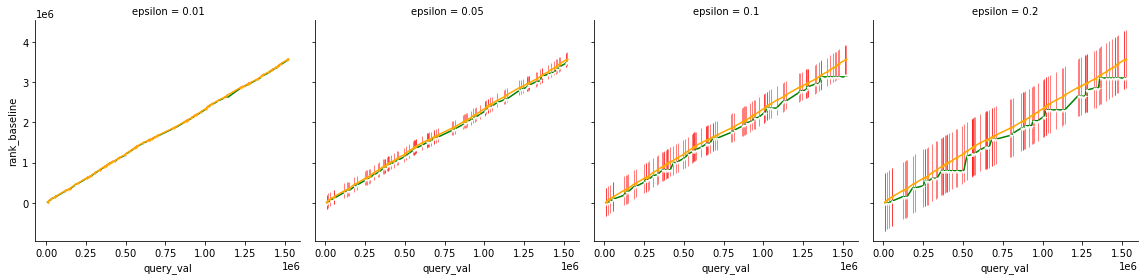
\includegraphics[width=.9\linewidth]{../../img/qdigest-erroplot_ecdf_RANK_t_0.png}
        \caption{Target 0}
        \label{fig:sub-first}
      \end{subfigure}
      \begin{subfigure}{.5\textwidth}
        \centering
        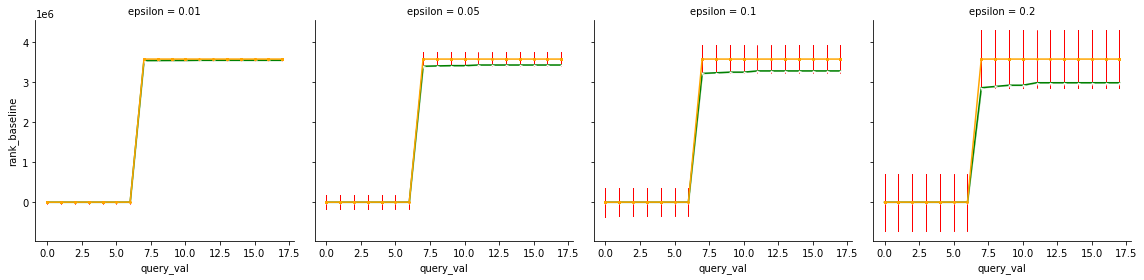
\includegraphics[width=.9\linewidth]{../../img/qdigest-erroplot_ecdf_RANK_t_3.png}
        \caption{Target 3}
      \end{subfigure}
      \caption{Barras de erro das queries do tipo \emph{rank}}
    \end{figure}
    
    \begin{figure}[H]
      \begin{subfigure}{.5\textwidth}
        \centering
        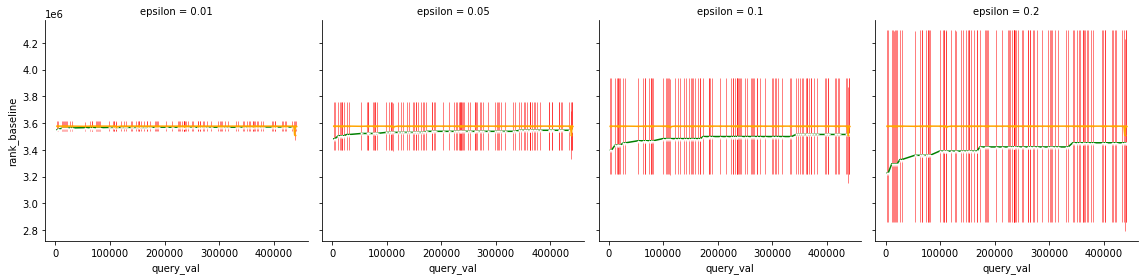
\includegraphics[width=.9\linewidth]{../../img/qdigest-erroplot_ecdf_RANK_t_4.png}
        \caption{Target 4}
        \label{fig:sub-first}
      \end{subfigure}
      \begin{subfigure}{.5\textwidth}
        \centering
        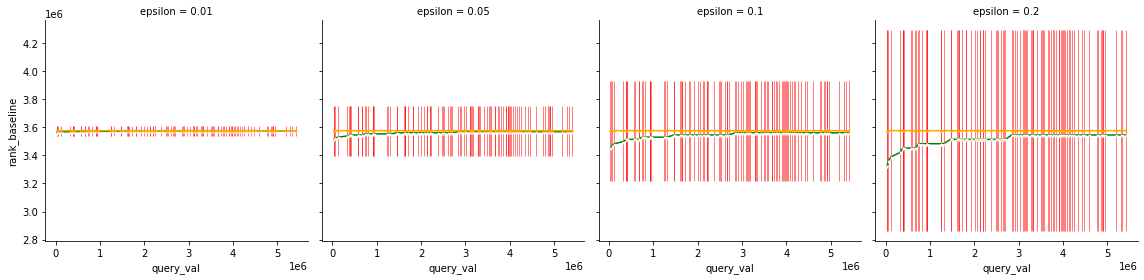
\includegraphics[width=.9\linewidth]{../../img/qdigest-erroplot_ecdf_RANK_t_5.png}
        \caption{Target 5}
      \end{subfigure}
      \caption{Barras de erro das queries do tipo \emph{rank}}
    \end{figure}

    \begin{figure}[H]
      \begin{subfigure}{.5\textwidth}
        \centering
        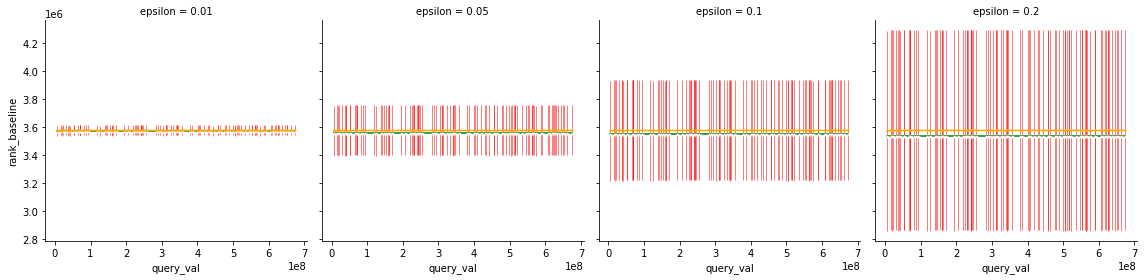
\includegraphics[width=.9\linewidth]{../../img/qdigest-erroplot_ecdf_RANK_t_6.png}
        \caption{Target 6}
        \label{fig:sub-first}
      \end{subfigure}
      \begin{subfigure}{.5\textwidth}
        \centering
        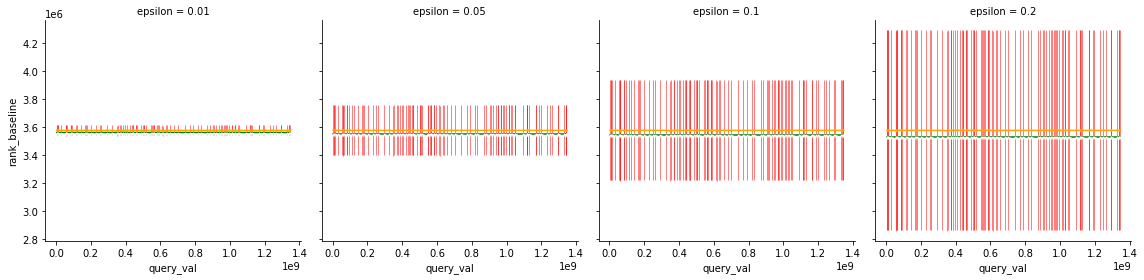
\includegraphics[width=.9\linewidth]{../../img/qdigest-erroplot_ecdf_RANK_t_7.png}
        \caption{Target 7}
      \end{subfigure}
      \caption{Barras de erro das queries do tipo \emph{rank}}
    \end{figure}

\end{document}
